\section*{Bài 1}

Biểu diễn phân số dưới dạng số thập phân tuần hoàn.
	
\addcontentsline{toc}{section}{Bài 1}

\begin{center}
    \textbf{\underline{Bài làm:}}
\end{center}

Để giải quyết bài toán, ta có thể sử dụng thư viện \textbf{NumberTheory} do \textbf{Maple} hỗ trợ. Thư viện này chứa các câu lệnh dùng để khảo sát các tính chất của số tự nhiên và số nguyên.\\
Câu lệnh \textbf{RepeatingDecimal($x$)} được sử dụng để biểu diễn một số hữu tỉ $x$  dưới dạng số thập phân tuần hoàn.\\
Có thể gọi câu lệnh với hai cách như sau:

\underline{\textbf{Cách 1:}} Sử dụng câu lệnh dài với đầy đủ tên thư viện và câu lệnh.

> \emph{NumberTheory:-RepeatingDecimal}($x$)

\underline{\textbf{Cách 2:}} Sử dụng câu lệnh ngắn bằng cách khai báo trước tên thư viện, sau đó gọi câu lệnh từ thư viện (khi dùng cách này, sau khi khai báo tên thư viện, ta có thể gọi bất kì câu lệnh nào từ thư viện đó, thao tác này  giúp rút gọn các dòng lệnh).

> \emph{with(NumberTheory):}

> \emph{RepeatingDecimal}($x$)

\textbf{Một số kết quả tính toán được khi sử dụng Maple:}

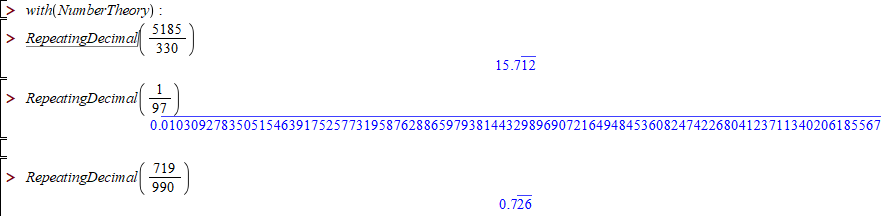
\includegraphics[width=1.0\textwidth]{bai1_maple.png}

\clearpage